\addcontentsline{toc}{subsection}{Slope Fields}
\subsection*{Slope Fields}

% slope fields as take home packet and extra examples

Slope Fields has been replaced with a take-home packet and quiz. This content will still be on the unit test but will not reviewed in class!! Link to Packet can be found below (clickable if using PDF version as well). Solutions can be found in the folder at start of book.

    \begin{center}
        
        
        \vspace{1cm}
        
        \qrcode{https://drive.google.com/file/d/1zI60e-JH81aCoSf6-0VDKDcLC84Jlf10/view?usp=sharing}
        
        \vspace{1cm}
        This is the same link that will appear on Canvas.
        
        \vspace{.5cm}
    \end{center}

\begin{questions}

    \question Find the equation of the curve that passes through the point $(1,\,3)$ and has a slope of $\displaystyle\frac{y}{x^2}$ at the point $(x,\,y)$, as shown in the graph below.
    
    \begin{flushright}
        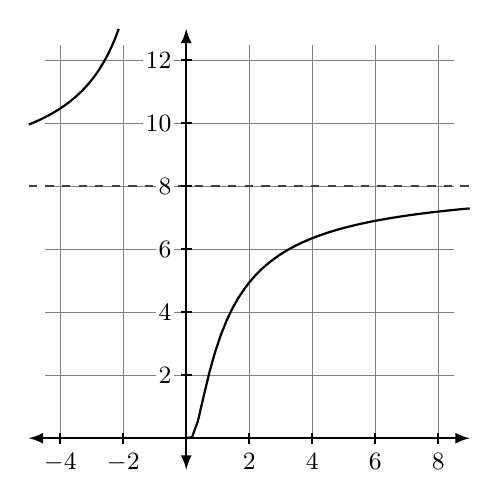
\begin{tikzpicture}[xscale=.4,yscale=.4,declare function={f(\x)=3*e^(1-(1/\x));} ,baseline=(current bounding box.north)]
            \draw[step=2,style=help lines,] (-4.5,0) grid (8.5,12.5);
            \draw[latex-latex, thick] (-5,0)--(9,0);
            \draw[latex-latex, thick] (0,-1)--(0,13);
            
            \draw[-,thick,dashed,color=gray!50!black] (-5,8) -- (9,8);
            
            \foreach \x in {-4,-2,2,4,6,8}
                \draw[thick] (\x,5pt) -- (\x,-5pt) node [below=.7mm,fill=white,inner sep=1pt] {\small$\x$};
            \foreach \y in {2,4,6,8,10,12}
                \draw[thick] (5pt,\y) -- (-5pt,\y) node [left=.7mm,fill=white,inner sep=1pt] {\small$\y$};
    
            
            \draw[thick] plot [samples=50,domain=.0001:9] ({\x},{f(\x)});
            \draw[thick] plot [samples=50,domain=-5:-2.1444] ({\x},{f(\x)});
            
            
        \end{tikzpicture}
    \end{flushright}
    
\end{questions}

\newpage

%add blurb about half carrying capicity is max growth rate for the DE.

